% =============================================
% CHAPITRE 6 — RÉALISATION ET DÉPLOIEMENT
% =============================================

\chapter{Réalisation et Déploiement}
\label{chap:realisation}
\vspace{1em}
\noindent\textbf{\large Sommaire}
\vspace{0.5em}
\localtableofcontents
\clearpage

Ce chapitre présente la réalisation concrète de la plateforme eKYC, de l'environnement de développement jusqu'au déploiement et à l'évaluation. Il décrit d'abord l'infrastructure applicative qui structure l'ensemble des composants, puis l'intégration des services IA au sein de cette infrastructure. Les interfaces client et administrateur, ainsi que l'évaluation de la conformité aux exigences de la Banque Centrale de Tunisie, complètent cette vision de bout en bout.

%=============================================================
\section{Environnement et outils de développement}
\label{sec:env-dev}
%=============================================================

Cette section présente l'ensemble des outils et technologies mobilisés pour la réalisation du projet, depuis l'environnement matériel et logiciel de développement jusqu'aux bibliothèques utilisées dans chaque couche du système.

\subsection{Environnement de développement}
\label{subsec:env-materiel}

L'ensemble du projet a été développé et testé sur un environnement local sous Windows 11. Aucun environnement cloud n'a été utilisé pour le développement applicatif, à l'exception de l'entraînement des modèles IA qui a nécessité des ressources GPU dédiées. Le Tableau~\ref{tab:ch6-env-materiel} présente la configuration matérielle utilisée.

\renewcommand{\arraystretch}{1.3}
\begin{longtable}{|p{5cm}|p{9.5cm}|}
  \rowcolor{bleu_principal}
  \textcolor{white}{\textbf{Composant}} & \textcolor{white}{\textbf{Détail}} \\
  \hline
  \endfirsthead
  \rowcolor{bleu_principal}
  \textcolor{white}{\textbf{Composant}} & \textcolor{white}{\textbf{Détail}} \\
  \hline
  \endhead
  Système d'exploitation & Windows 11 Home 64 bits \\ \hline
  Processeur             & AMD Ryzen 5 5600H --- 3.30 GHz \\ \hline
  Mémoire RAM            & 16 Go (13,9 Go utilisable) \\ \hline
  GPU principal          & NVIDIA GeForce RTX 3050 Ti Laptop GPU --- 4 Go VRAM \\ \hline
  GPU intégré            & AMD Radeon Graphics --- 2 Go \\ \hline
  Stockage               & 477 Go SSD \\ \hline
  \caption{Configuration matérielle de l'environnement de développement}
  \label{tab:ch6-env-materiel}
\end{longtable}

Le GPU NVIDIA RTX 3050 Ti a été utilisé pour l'inférence des modèles YOLOv11m et PaddleOCR en local. L'entraînement des modèles, plus gourmand en ressources, a été réalisé sur Google Colab pour bénéficier de GPU T4/A100 plus puissants.

\subsection{Outils de développement}
\label{subsec:outils-dev}

Les outils présentés dans cette sous-section couvrent l'édition de code, la conception des interfaces, la gestion des données et l'entraînement des modèles IA.

\renewcommand{\arraystretch}{1.3}
\begin{longtable}{|p{4cm}|p{10.5cm}|}
  \rowcolor{bleu_principal}
  \textcolor{white}{\textbf{Outil}} & \textcolor{white}{\textbf{Rôle}} \\
  \hline
  \endfirsthead
  \rowcolor{bleu_principal}
  \textcolor{white}{\textbf{Outil}} & \textcolor{white}{\textbf{Rôle}} \\
  \hline
  \endhead
  Visual Studio Code  & Éditeur principal pour le développement backend, frontend et services IA \\ \hline
  Figma               & Conception des interfaces utilisateur (maquettes client et dashboard admin) \\ \hline
  DBeaver             & Visualisation et gestion de la base de données PostgreSQL en local \\ \hline
  PostgreSQL          & Base de données relationnelle principale \\ \hline
  MinIO               & Serveur de stockage de fichiers local (images, documents, selfies) \\ \hline
  Google Colab        & Entraînement des modèles YOLOv11m sur GPU (T4 / A100) \\ \hline
  Roboflow            & Annotation des datasets d'images (CIN recto, CIN verso, passeport) et export au format YOLO \\ \hline
  \caption{Outils de développement utilisés}
  \label{tab:ch6-outils}
\end{longtable}

\subsection{Bibliothèques et frameworks}
\label{subsec:bibliotheques}

Le système est organisé en plusieurs couches techniques, chacune s'appuyant sur un ensemble de bibliothèques spécialisées. Les tableaux suivants les présentent couche par couche.

\subsubsection{Frontend}

\renewcommand{\arraystretch}{1.3}
\begin{longtable}{|p{3.5cm}|p{1.5cm}|p{9.5cm}|}
  \rowcolor{bleu_principal}
  \textcolor{white}{\textbf{Bibliothèque}} & \textcolor{white}{\textbf{Version}} & \textcolor{white}{\textbf{Rôle}} \\
  \hline
  \endfirsthead
  \rowcolor{bleu_principal}
  \textcolor{white}{\textbf{Bibliothèque}} & \textcolor{white}{\textbf{Version}} & \textcolor{white}{\textbf{Rôle}} \\
  \hline
  \endhead
  Next.js         & 14.2      & Framework React — interface client et dashboard admin \\ \hline
  TypeScript      & 5         & Typage statique \\ \hline
  Tailwind CSS    & 3.4       & Styles et mise en page \\ \hline
  Lucide React    & 1.14      & Bibliothèque d'icônes \\ \hline
  react-webcam    & 7.2       & Accès à la caméra du client dans le navigateur \\ \hline
  next-auth       & 5.0 beta  & Gestion des sessions d'authentification \\ \hline
  \caption{Bibliothèques frontend}
  \label{tab:ch6-frontend}
\end{longtable}

\subsubsection{Backend (Python 3.11 64 bits)}

\renewcommand{\arraystretch}{1.3}
\begin{longtable}{|p{4.5cm}|p{10cm}|}
  \rowcolor{bleu_principal}
  \textcolor{white}{\textbf{Bibliothèque}} & \textcolor{white}{\textbf{Rôle}} \\
  \hline
  \endfirsthead
  \rowcolor{bleu_principal}
  \textcolor{white}{\textbf{Bibliothèque}} & \textcolor{white}{\textbf{Rôle}} \\
  \hline
  \endhead
  FastAPI                    & Framework API REST --- routes, validation, documentation automatique \\ \hline
  SQLAlchemy                 & ORM --- mapping des modèles Python vers les tables PostgreSQL \\ \hline
  Alembic                    & Migrations de schéma base de données \\ \hline
  Pydantic                   & Validation des données entrantes et sortantes \\ \hline
  python-jose                & Génération et vérification des tokens JWT \\ \hline
  passlib / bcrypt           & Hachage sécurisé des mots de passe \\ \hline
  httpx                      & Appels HTTP vers les services IA \\ \hline
  minio                      & Client Python pour le stockage MinIO \\ \hline
  redis                      & Client Python pour la blacklist des tokens JWT \\ \hline
  loguru                     & Journalisation des logs applicatifs \\ \hline
  jellyfish / doublemetaphone & Comparaison phonétique des noms pour le filtrage AML \\ \hline
  \caption{Bibliothèques backend}
  \label{tab:ch6-backend}
\end{longtable}

\subsubsection{Services IA}

\renewcommand{\arraystretch}{1.3}
\begin{longtable}{|p{4.5cm}|p{10cm}|}
  \rowcolor{bleu_principal}
  \textcolor{white}{\textbf{Bibliothèque}} & \textcolor{white}{\textbf{Rôle}} \\
  \hline
  \endfirsthead
  \rowcolor{bleu_principal}
  \textcolor{white}{\textbf{Bibliothèque}} & \textcolor{white}{\textbf{Rôle}} \\
  \hline
  \endhead
  Ultralytics (YOLOv11) & Détection des zones de champs sur les documents et détection visage \\ \hline
  OpenCV                & Traitement d'images (redimensionnement, conversion, crop) \\ \hline
  Pillow                & Manipulation des images Python \\ \hline
  NumPy                 & Calculs matriciels sur les images \\ \hline
  websockets            & Communication WebSocket temps réel pour la capture guidée \\ \hline
  PaddleOCR             & Moteur de reconnaissance de caractères (arabe + français) \\ \hline
  PaddlePaddle GPU      & Framework deep learning sous-jacent de PaddleOCR --- exécution sur GPU \\ \hline
  face-recognition      & Comparaison des embeddings biométriques entre deux visages \\ \hline
  \caption{Bibliothèques des services IA}
  \label{tab:ch6-ia}
\end{longtable}

\subsection{Gestion du projet}
\label{subsec:gestion-projet}

\renewcommand{\arraystretch}{1.3}
\begin{longtable}{|p{4cm}|p{10.5cm}|}
  \rowcolor{bleu_principal}
  \textcolor{white}{\textbf{Outil}} & \textcolor{white}{\textbf{Rôle}} \\
  \hline
  \endfirsthead
  \rowcolor{bleu_principal}
  \textcolor{white}{\textbf{Outil}} & \textcolor{white}{\textbf{Rôle}} \\
  \hline
  \endhead
  Turborepo & Orchestration du monorepo --- gestion des dépendances et des tâches de build entre les applications \\ \hline
  Git       & Gestion de versions du code source \\ \hline
  \caption{Outils de gestion du projet}
  \label{tab:ch6-gestion}
\end{longtable}


%=============================================================
\section{Infrastructure applicative}
\label{sec:infrastructure-applicative}
%=============================================================

La mise en œuvre de la plateforme eKYC repose sur une infrastructure applicative structurée en trois niveaux complémentaires : une architecture globale qui organise l'ensemble des composants, une API REST qui expose les fonctionnalités métier, et deux systèmes de persistance distincts pour les données structurées et les fichiers binaires. Cette section décrit chacun de ces niveaux.

\subsection{Architecture globale de la plateforme}
\label{subsec:archi-globale}

La plateforme eKYC est structurée en \textbf{monorepo Turborepo}, regroupant dans un seul dépôt Git l'ensemble des applications et services du système. Cette organisation centralise la gestion des dépendances, facilite le partage de types communs et garantit la cohérence des versions entre les différentes couches de l'application, comme illustré dans la Figure~\ref{fig:ch6-archi-globale}.

\vspace{0.6em}
\begin{center}
  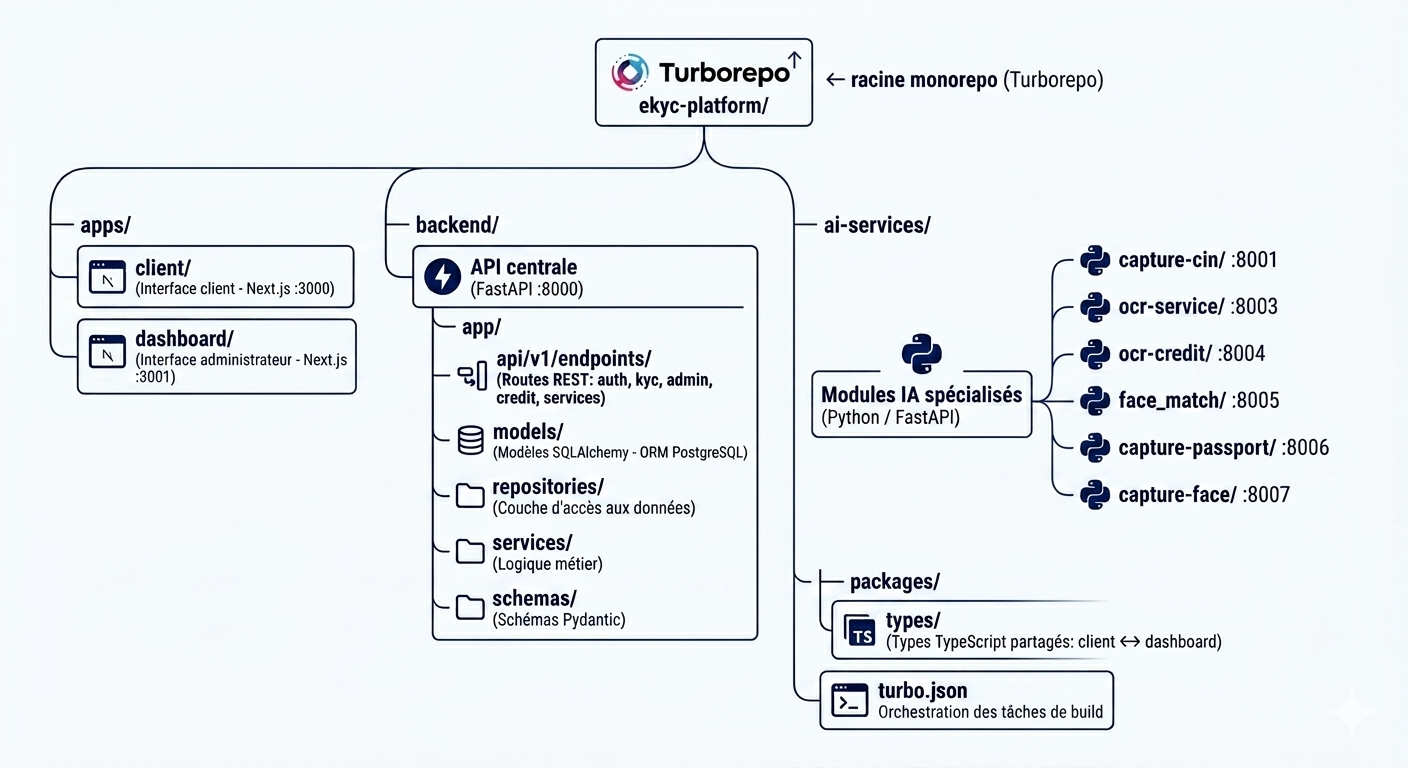
\includegraphics[width=0.95\textwidth]{images/image_ch5/archi_globale.png}
  \captionof{figure}{Architecture globale de la plateforme eKYC}
  \label{fig:ch6-archi-globale}
\end{center}
\vspace{0.6em}

La plateforme comprend deux applications frontend distinctes dont les métiers sont suffisamment différenciés pour justifier une séparation complète : l'une dédiée au parcours client, l'autre aux agents et superviseurs. Un backend central FastAPI orchestre les deux interfaces et prend en charge l'ensemble de la logique métier : gestion des dossiers KYC, authentification, filtrage AML et persistance. En complément, un système IA regroupe sept services spécialisés appelés directement par le frontend, indépendamment du backend. Les sections suivantes détaillent les points d'entrée de ce backend ainsi que les mécanismes de persistance sur lesquels il s'appuie.

\subsection{API REST --- Endpoints principaux}
\label{subsec:api-rest}

Le backend expose une API REST versionnée sous le préfixe \texttt{/api/v1}, organisée en six groupes de routes selon le domaine fonctionnel. Le Tableau~\ref{tab:api-routes} présente la vue d'ensemble de ces groupes.

\renewcommand{\arraystretch}{1.3}
\begin{longtable}{|p{2cm}|p{4cm}|p{6cm}|p{3cm}|}
  \rowcolor{bleu_principal}
  \textcolor{white}{\textbf{Groupe}} & \textcolor{white}{\textbf{Préfixe}} & \textcolor{white}{\textbf{Rôle}} & \textcolor{white}{\textbf{Acteur}} \\
  \hline
  \endfirsthead
  \rowcolor{bleu_principal}
  \textcolor{white}{\textbf{Groupe}} & \textcolor{white}{\textbf{Préfixe}} & \textcolor{white}{\textbf{Rôle}} & \textcolor{white}{\textbf{Acteur}} \\
  \hline
  \endhead
  \textbf{Auth}     & \texttt{/api/v1/auth}     & Authentification, inscription, gestion des tokens & Client + Admin \\
  \hline
  \textbf{KYC}      & \texttt{/api/v1/kyc}      & Soumission et suivi des demandes KYC              & Client \\
  \hline
  \textbf{Admin}    & \texttt{/api/v1/admin}    & Revue, validation, scoring, alertes AML           & Agent / Superviseur / Admin \\
  \hline
  \textbf{Crédit}   & \texttt{/api/v1/credit}   & Demandes de crédit bancaire                       & Client + Admin \\
  \hline
  \textbf{Services} & \texttt{/api/v1/services} & Demandes de carte bancaire et chéquier            & Client + Admin \\
  \hline
  \textbf{IA}       & \texttt{/api/v1/admin/ia} & Métriques IA en temps réel (monitoring)           & Superviseur \\
  \hline
  \caption{Vue d'ensemble des groupes de routes --- API REST}
  \label{tab:api-routes}
\end{longtable}

Ces six groupes de routes couvrent l'ensemble des interactions entre les interfaces et le backend. Les données produites par ces échanges — qu'il s'agisse de résultats OCR, de décisions d'agents ou de scores de risque — sont ensuite persistées dans les deux systèmes décrits ci-après.

\subsection{Persistance et stockage}
\label{subsec:persistance-stockage}

La plateforme repose sur deux systèmes de persistance complémentaires : \textbf{PostgreSQL} pour les données structurées et \textbf{MinIO} pour les fichiers binaires. Les deux sous-sections suivantes décrivent le rôle et le contenu de chacun.

\subsubsection{Base de données PostgreSQL}

PostgreSQL est la base de données relationnelle principale du système. Toutes les données métier y sont persistées : comptes utilisateurs, demandes KYC, résultats OCR, décisions administratives, journaux d'audit et listes de filtrage AML. Le Tableau~\ref{tab:bdd-tables} présente les tables principales du schéma.

\renewcommand{\arraystretch}{1.3}
\begin{longtable}{|p{5cm}|p{9.5cm}|}
  \rowcolor{bleu_principal}
  \textcolor{white}{\textbf{Table}} & \textcolor{white}{\textbf{Contenu}} \\
  \hline
  \endfirsthead
  \rowcolor{bleu_principal}
  \textcolor{white}{\textbf{Table}} & \textcolor{white}{\textbf{Contenu}} \\
  \hline
  \endhead
  \texttt{users}                       & Comptes utilisateurs (client, agent, superviseur, admin) \\ \hline
  \texttt{user\_information}           & Données d'identité KYC du client (nom, CIN, date de naissance...) \\ \hline
  \texttt{kyc\_demandes}               & Demandes KYC avec statut, type de compte, agent assigné, niveau de risque \\ \hline
  \texttt{kyc\_documents}              & Documents soumis (CIN recto/verso, passeport) avec URL MinIO \\ \hline
  \texttt{ocr\_results}                & Résultats bruts YOLO + PaddleOCR en JSONB (structured, raw\_detections, scores) \\ \hline
  \texttt{ocr\_corrections}            & Corrections manuelles des champs OCR (client ou agent) \\ \hline
  \texttt{selfies}                     & URLs MinIO des selfies capturés \\ \hline
  \texttt{face\_crops}                 & URLs MinIO des crops visage extraits par YOLO \\ \hline
  \texttt{validation\_scores}          & Score de risque global calculé par le backend \\ \hline
  \texttt{blacklist}                   & Liste noire AML (noms, CIN) \\ \hline
  \texttt{ppe\_list}                   & Liste des Personnes Politiquement Exposées \\ \hline
  \texttt{blacklist\_matches}          & Correspondances détectées entre un client et la blacklist \\ \hline
  \texttt{ppe\_matches}                & Correspondances PPE détectées \\ \hline
  \texttt{identity\_duplicate\_alerts} & Alertes de doublons biométriques ou d'identité entre dossiers \\ \hline
  \texttt{demand\_comments}            & Commentaires internes des agents sur les dossiers \\ \hline
  \texttt{audit\_logs}                 & Journal des actions sensibles (connexion, décision, modification) \\ \hline
  \texttt{audit\_views}                & Historique des consultations de dossiers par les agents \\ \hline
  \texttt{comptes\_bancaires}          & Comptes bancaires ouverts au nom des clients \\ \hline
  \texttt{demand\_credit}              & Demandes de crédit bancaire \\ \hline
  \texttt{demande\_carte}              & Demandes de carte bancaire \\ \hline
  \texttt{demande\_chequier}           & Demandes de chéquier \\ \hline
  \caption{Schéma des tables principales --- PostgreSQL}
  \label{tab:bdd-tables}
\end{longtable}

PostgreSQL centralise ainsi toutes les informations métier sous forme structurée. Les fichiers binaires associés à ces enregistrements sont quant à eux gérés par un système dédié, présenté ci-après.

\subsubsection{Stockage objet MinIO}

Si PostgreSQL gère les données structurées, les fichiers binaires — images de documents, selfies, crops de visage — sont pris en charge par MinIO. Dans le cadre de ce projet, MinIO est déployé en tant que serveur de stockage local dédié, simulant le comportement d'un serveur institutionnel tel que celui qu'une banque exploiterait en production pour archiver les documents sensibles de ses clients. Ce choix répond à une contrainte de sécurité fondamentale : aucune image ne doit transiter vers un service externe ou un stockage cloud tiers. Toutes les images restent confinées à l'infrastructure locale, garantissant la souveraineté des données conformément aux exigences du secteur bancaire.

MinIO expose une interface compatible S3 qui permet à chaque service IA d'y accéder directement via une URL interne. Chaque image capturée pendant le parcours KYC y est enregistrée dès sa production et référencée dans PostgreSQL par son adresse. Le Tableau~\ref{tab:minio-categories} présente les catégories d'images stockées.

\renewcommand{\arraystretch}{1.3}
\begin{longtable}{|p{4cm}|p{10cm}|}
  \rowcolor{bleu_principal}
  \textcolor{white}{\textbf{Catégorie}} & \textcolor{white}{\textbf{Contenu}} \\
  \hline
  \endfirsthead
  \rowcolor{bleu_principal}
  \textcolor{white}{\textbf{Catégorie}} & \textcolor{white}{\textbf{Contenu}} \\
  \hline
  \endhead
  Documents d'identité & Photos de la CIN (recto et verso) ou du passeport capturées par le client \\ \hline
  Selfies              & Photo du visage prise lors de l'étape de vérification biométrique \\ \hline
  Crops visage         & Zone du visage découpée automatiquement depuis le document d'identité \\ \hline
  Documents financiers & Attestations de salaire pour les demandes de crédit \\ \hline
  \caption{Catégories d'images stockées dans MinIO}
  \label{tab:minio-categories}
\end{longtable}

PostgreSQL et MinIO jouent ainsi des rôles complémentaires sans être directement connectés : PostgreSQL conserve les \textbf{informations} sur chaque dossier, MinIO conserve les \textbf{fichiers}. Le lien entre les deux se fait par les URLs — chaque image stockée dans MinIO est référencée dans PostgreSQL par son adresse. Lorsqu'un agent consulte un dossier, le backend récupère les métadonnées depuis PostgreSQL puis charge les images directement depuis MinIO. Cette complémentarité constitue le socle sur lequel repose l'intégration des services IA, décrite dans la section suivante.


%=============================================================
\section{Intégration des services IA}
\label{sec:integration-ia}
%=============================================================

L'infrastructure applicative étant posée, cette section décrit comment les services IA développés lors du premier incrément s'y intègrent pour former un système unifié. Elle présente d'abord la stratégie d'intégration par contrat d'interface, puis détaille les flux de communication effectifs entre chaque couche du système.

\subsection{De deux incréments à un système unifié}
\label{subsec:integration-increments}

Le développement de la plateforme eKYC a suivi deux incréments parallèles et complémentaires : un incrément dédié aux modules d'intelligence artificielle (capture, OCR, comparaison biométrique) et un incrément dédié au système applicatif (backend, interfaces client et administrateur, base de données). Menés de façon indépendante, ces deux incréments convergent à la soumission du dossier KYC pour former un \textbf{système eKYC unifié} : le pipeline IA produit les données d'identité et les scores biométriques, le système applicatif les reçoit, les persiste et les soumet à la décision d'un agent. La question centrale de l'intégration était de définir comment ces deux incréments allaient se rejoindre sans créer de dépendance forte entre eux. Les trois sous-sections suivantes décrivent respectivement le contrat d'interface retenu, le point de jonction effectif, et les bénéfices de cette approche.

\subsubsection{Le contrat d'interface comme point de jonction}

La décision fondamentale a été de définir un \textbf{contrat d'interface clair} entre les deux incréments avant même de commencer le développement. Ce contrat repose sur un principe simple : le système IA ne connaît pas le système applicatif, et le système applicatif ne connaît pas les modèles IA. Les deux communiquent uniquement par échange de données structurées (JSON) et d'adresses d'images (URLs MinIO), comme illustré par la Figure~\ref{fig:ch6-contrat-interface}.

\vspace{0.6em}
\begin{center}
  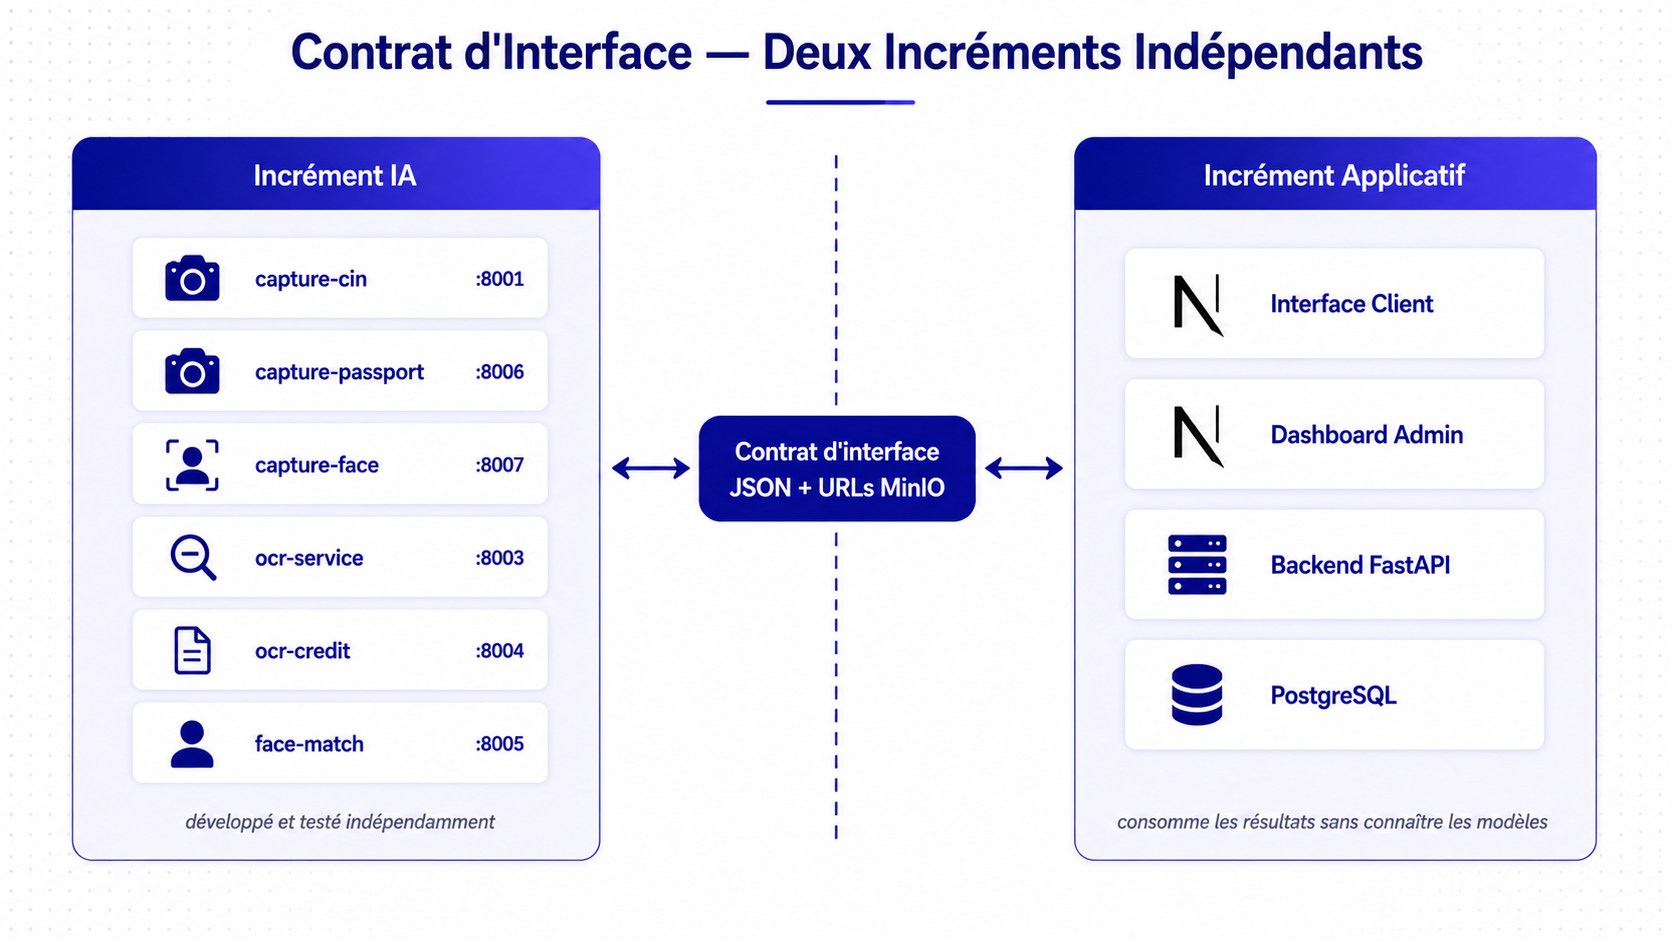
\includegraphics[width=0.95\textwidth]{images/image-ch6/Diagramme de contrat d'interface système.png}
  \captionof{figure}{Contrat d'interface entre le système IA et le système applicatif}
  \label{fig:ch6-contrat-interface}
\end{center}
\vspace{0.6em}

Concrètement, chaque module IA expose un endpoint précis avec un format de réponse fixe. Le système applicatif consomme ces réponses sans se préoccuper de ce qui se passe à l'intérieur du module. Ce découplage a permis aux deux incréments d'avancer indépendamment : le système applicatif pouvait être développé et testé avec des données simulées pendant que les modèles IA étaient encore en cours d'entraînement.

\subsubsection{Comment les deux incréments se rejoignent}

Fort de ce contrat d'interface, le point de jonction effectif entre les deux incréments est l'endpoint \texttt{POST /api/v1/kyc/submit-full} du backend. C'est à ce moment que les résultats produits par le système IA (données d'identité extraites, scores de confiance, URL du crop visage) sont transmis au système applicatif pour être persistés et soumis à la validation d'un agent, comme illustré par la Figure~\ref{fig:ch6-jonction-increments}.

\vspace{0.6em}
\begin{center}
  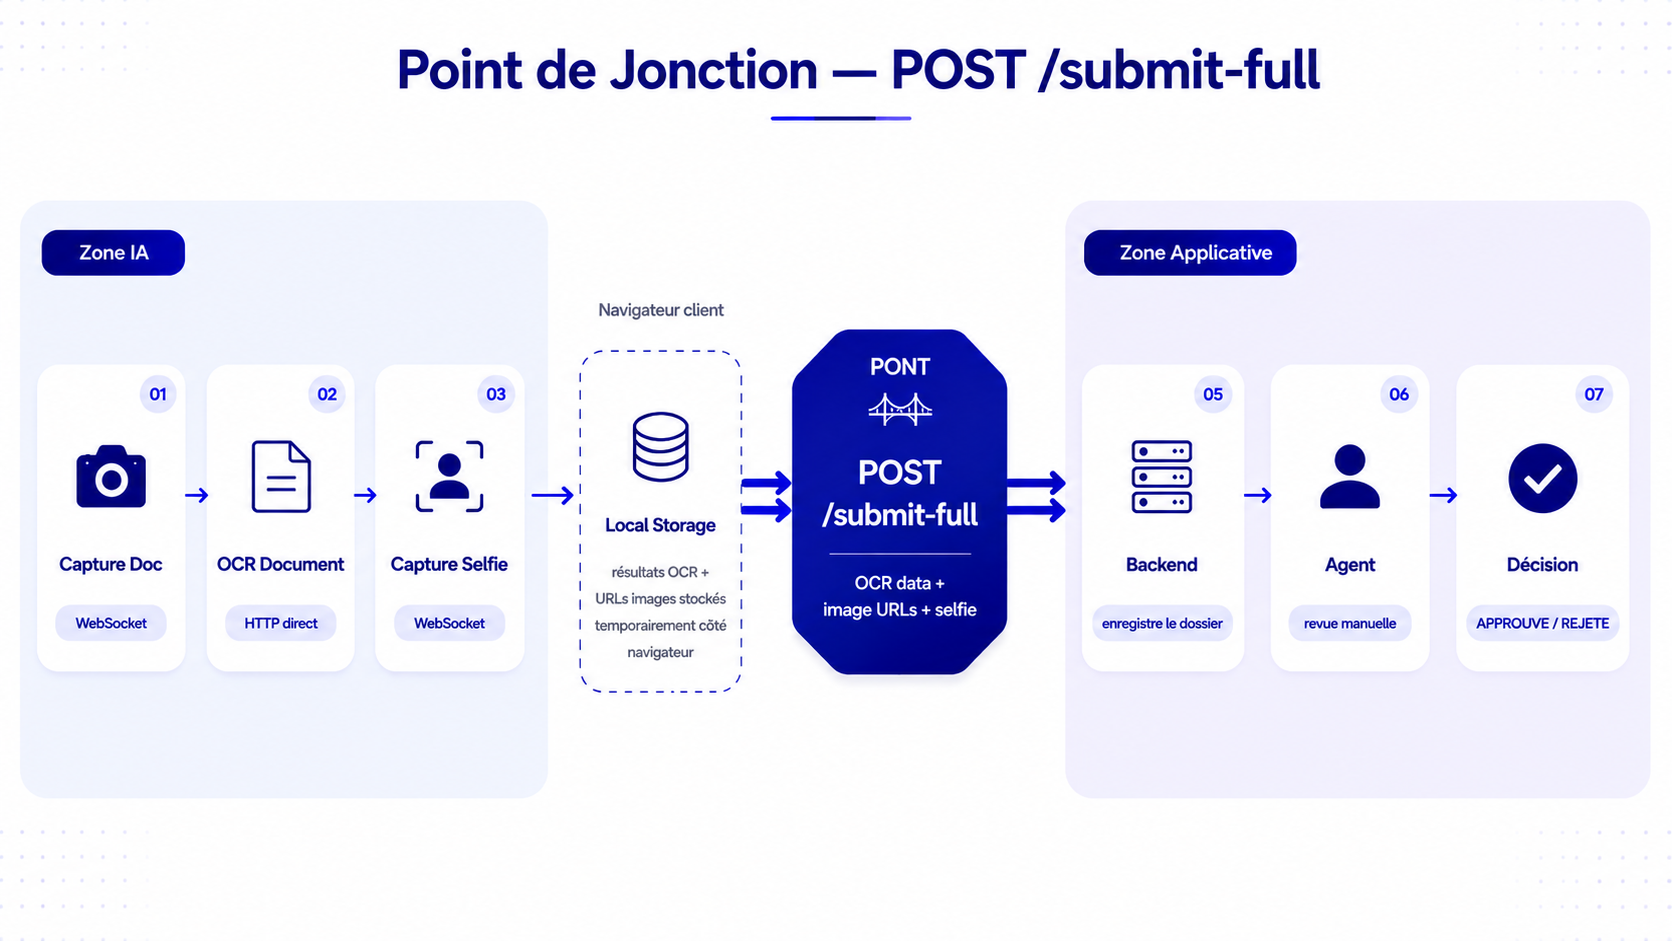
\includegraphics[width=0.95\textwidth]{images/image-ch6/ChatGPT Image 30 mai 2026, 03_02_18.png}
  \captionof{figure}{Point de jonction entre les deux incréments --- soumission finale du dossier KYC}
  \label{fig:ch6-jonction-increments}
\end{center}
\vspace{0.6em}

Jusqu'à ce point, l'interface client orchestre les appels aux modules IA, collecte leurs résultats étape par étape et les conserve localement. Ce n'est qu'à cet instant que le système applicatif prend le relais : il enregistre le dossier, assigne un agent et déclenche le processus de validation.

\subsubsection{Bénéfices de cette approche}

Ce mode d'intégration a apporté deux avantages concrets pendant le développement. D'abord, il a été possible de tester chaque incrément séparément : les modules IA pouvaient être évalués sur des jeux d'images indépendamment du backend, et le backend pouvait être développé avec des données OCR fictives avant que les vrais modèles soient prêts. Ensuite, cette séparation rend le système évolutif : remplacer un modèle OCR par une version plus performante ne nécessite aucune modification du backend, tant que le format de la réponse reste identique.

Cette stratégie d'intégration étant posée, la sous-section suivante détaille les flux de communication effectifs entre chaque couche du système au moment de l'exécution.

%-------------------------------------------------------------
\subsection{Communication entre les couches}
\label{subsec:communication-couches}

Au-delà du contrat d'interface qui définit les formats d'échange, le système IA est structuré en un ensemble de modules indépendants, chacun accessible via une adresse réseau locale dédiée. Cette organisation permet de faire évoluer, remplacer ou redémarrer un module sans affecter les autres composants du système. La Figure~\ref{fig:ch6-communication-ia} illustre les flux de communication entre chaque couche, présentés dans les paragraphes qui suivent.

\vspace{0.6em}
\begin{center}
  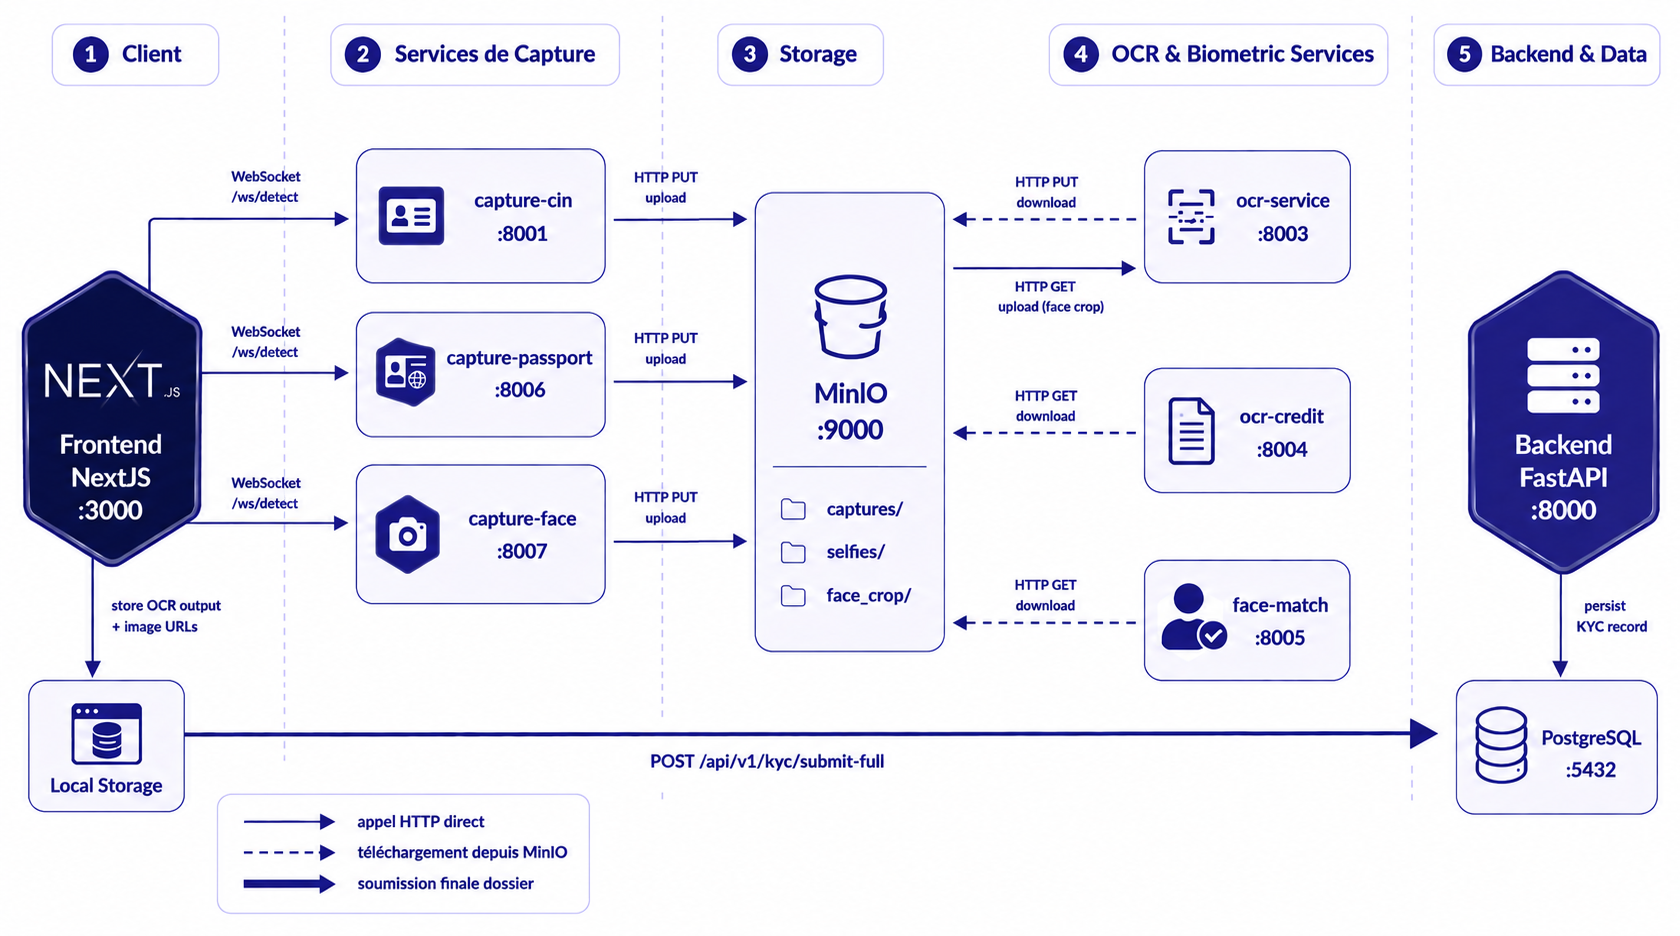
\includegraphics[width=0.95\textwidth]{images/image_ch5/communicationIa.png}
  \captionof{figure}{Schéma de communication entre les couches de la plateforme eKYC}
  \label{fig:ch6-communication-ia}
\end{center}
\vspace{0.6em}

\paragraph{L'interface client}
est le point de départ de toutes les interactions. Elle contacte directement les modules de capture pour guider le client devant sa caméra, puis les modules OCR pour extraire les informations des documents photographiés, sans jamais passer par le backend pour ces opérations. Ce choix réduit la latence et évite de surcharger le serveur central avec des flux vidéo ou des images volumineuses.

\paragraph{Les modules de capture}
(CIN, passeport, selfie) reçoivent les images de la caméra en temps réel, détectent la présence et la qualité du document dans le cadre, et déposent l'image directement dans MinIO une fois la capture validée par le client. Ils retournent à l'interface l'adresse URL de l'image stockée, sans jamais transmettre l'image elle-même au backend.

\paragraph{Les modules OCR}
reçoivent ces adresses d'images depuis l'interface, téléchargent les images depuis MinIO, analysent le document pour en extraire les champs textuels, et retournent les données structurées à l'interface. Le résultat est conservé temporairement côté client jusqu'à la soumission du dossier.

\paragraph{Le backend}
n'intervient qu'à deux moments précis : lors de la soumission du dossier, où il reçoit en une seule requête l'ensemble des données collectées par l'interface ; et lors de la validation par un agent, où il sollicite le module de comparaison biométrique.

\paragraph{Le module de comparaison biométrique}
est le seul service IA appelé exclusivement par le backend : il compare le visage extrait du document avec le selfie pour détecter toute tentative d'usurpation d'identité entre plusieurs dossiers.

MinIO joue un rôle transversal à l'ensemble de ces échanges, comme détaillé ci-après.

\subsubsection{Rôle de MinIO comme intermédiaire universel}

Transversalement à toutes ces couches, MinIO constitue le seul point de passage des images entre tous les acteurs du système. Aucune image n'est transmise directement d'un service à un autre sous forme de fichier — chaque composant dépose ou récupère les images via MinIO en utilisant une adresse URL. Cette approche simplifie les échanges, évite de transférer des fichiers volumineux dans les requêtes réseau, et garantit que chaque image est archivée de façon centralisée dès sa création.

%=============================================================
\section{Interface client}
\label{sec:interface-client}
%=============================================================

% [Contenu à rédiger ultérieurement]


%=============================================================
\section{Interface administrateur}
\label{sec:interface-admin}
%=============================================================

% [Contenu à rédiger ultérieurement]



\section*{Conclusion du chapitre}

Ce chapitre a présenté la réalisation complète de la plateforme eKYC, de l'infrastructure applicative jusqu'à l'intégration des services IA. L'ensemble des composants développés dans les deux incréments --- le pipeline d'intelligence artificielle d'une part, et le système applicatif d'autre part --- se rejoignent à la soumission finale du dossier pour former un \textbf{système eKYC unifié et opérationnel} : le client est guidé par le pipeline IA à chaque étape de capture, ses données sont extraites et vérifiées automatiquement, puis transmises au backend qui orchestre la validation par un agent selon les exigences de la Banque Centrale de Tunisie. Le résultat est une plateforme cohérente, où les deux incréments ne font plus qu'un seul système au service du parcours d'ouverture de compte.
